\documentclass[12pt, letterpaper]{article}
\title{Lab Report A2}
\usepackage{graphicx}
\usepackage{amsmath}
\usepackage[margin=1in]{geometry}% Sets 1in margins. 
\usepackage{fancyhdr}			% Creates headers and footers
\usepackage{enumerate}          %These two package give custom labels to
\usepackage[shortlabels]{enumitem}
\author{Aditya Gupta}
\date{\today}
\begin{document}
\maketitle
\newpage
\tableofcontents
\newpage
\section{Introduction}
This lab report explores the data procured by measuring the distance travelled by a toy car at regular time intervals in an aim to determine the speed of said car.
\section{Raw Data}
The following table contains the data for the collected experiment
\begin{table}[h!]
\centering
\begin{tabular}{|c|c|c|c|c|}
\hline
\textbf{Time(s)} & \textbf{Trial 1 (cm)} & \textbf{Trial 2 (cm)} & \textbf{Trial 3 (cm)} & \textbf{Trial 4 (cm)} \\ \hline
1                & 18.7       & 24.5       & 24.4       & 21         \\ \hline
2                & 42         & 43.1       & 44.5       & 40.4       \\ \hline
3                & 64.6       & 64.5       & 60.7       & 60.1       \\ \hline
4                & 82.6       & 79         & 77.5       & 80.3       \\ \hline
5                & 102.6      & 97.4       & 98.4       & 99.2       \\ \hline
6                & 122.1      & 116.9      & 117        & 118.5      \\ \hline
\end{tabular}
\caption{Data table for all trials}
\end{table}
\section{Processed Data}
The first step to processing the data is to obtain the mean of all observations. Here is a sample calculation:
\[
\Sigma_{i=0}^n (d) =\frac{18.7+24.5+24.4+21}{4} = 22.2
\]
Calculating all averages,
\begin{table}[h!]
\centering
\begin{tabular}{|c|c|c|c|c|c|}
\hline
\textbf{Time(s)} & \textbf{Trial 1 (cm)} & \textbf{Trial 2 (cm)} & \textbf{Trial 3 (cm)} & \textbf{Trial 4 (cm)} & \textbf{Average (cm)} \\ \hline
1                & 18.7       & 24.5       & 24.4       & 21         & 22.2        \\ \hline
2                & 42         & 43.1       & 44.5       & 40.4       & 42.5        \\ \hline
3                & 64.6       & 64.5       & 60.7       & 60.1       & 62.5        \\ \hline
4                & 82.6       & 79         & 77.5       & 80.3       & 79.9        \\ \hline
5                & 102.6      & 97.4       & 98.4       & 99.2       & 99.4        \\ \hline
6                & 122.1      & 116.9      & 117        & 118.5      & 118.6       \\ \hline
\end{tabular}
\caption{Data table with average values for each time point.}
\end{table}

Now, to calculate Random Uncertainty in the Data:

\[
\text{Random Uncertainty} = \frac{Max - Min}{2} 
\]
For the 1 second intervals:
\[
\text{Random Uncertainty} = \frac{24.5 -18.7}{2} = 2.9
\]
Calculating random uncertainties for all second intervals:

\begin{table}[h!]
\centering
\small
\begin{tabular}
{|@{}c@{}|@{}c@{}|@{}c@{}|@{}c@{}|@{}c@{}|@{}c@{}|@{}c@{}|@{}}
\hline
\textbf{Time(s)} & \textbf{Trial 1(cm)} & \textbf{Trial 2(cm)} & \textbf{Trial 3(cm)} & \textbf{Trial 4(cm)} & \textbf{Average(cm)} & \textbf{Random Uncertainty(cm)} \\ \hline
1                & 18.7                  & 24.5                  & 24.4                  & 21                    & 22.2                  & 2.9                               \\ \hline
2                & 42                    & 43.1                  & 44.5                  & 40.4                  & 42.5                  & 2.05                              \\ \hline
3                & 64.6                  & 64.5                  & 60.7                  & 60.1                  & 62.5                  & 2.25                              \\ \hline
4                & 82.6                  & 79                    & 77.5                  & 80.3                  & 79.9                  & 2.55                              \\ \hline
5                & 102.6                 & 97.4                  & 98.4                  & 99.2                  & 99.4                  & 2.6                               \\ \hline
6                & 122.1                 & 116.9                 & 117                   & 118.5                 & 118.6                 & 2.6                               \\ \hline
\end{tabular}

\caption{Data table with average values and random uncertainty for each time point.}
\end{table}

\section{Graphing and Calculation of Slopes}
\subsection{Graph}
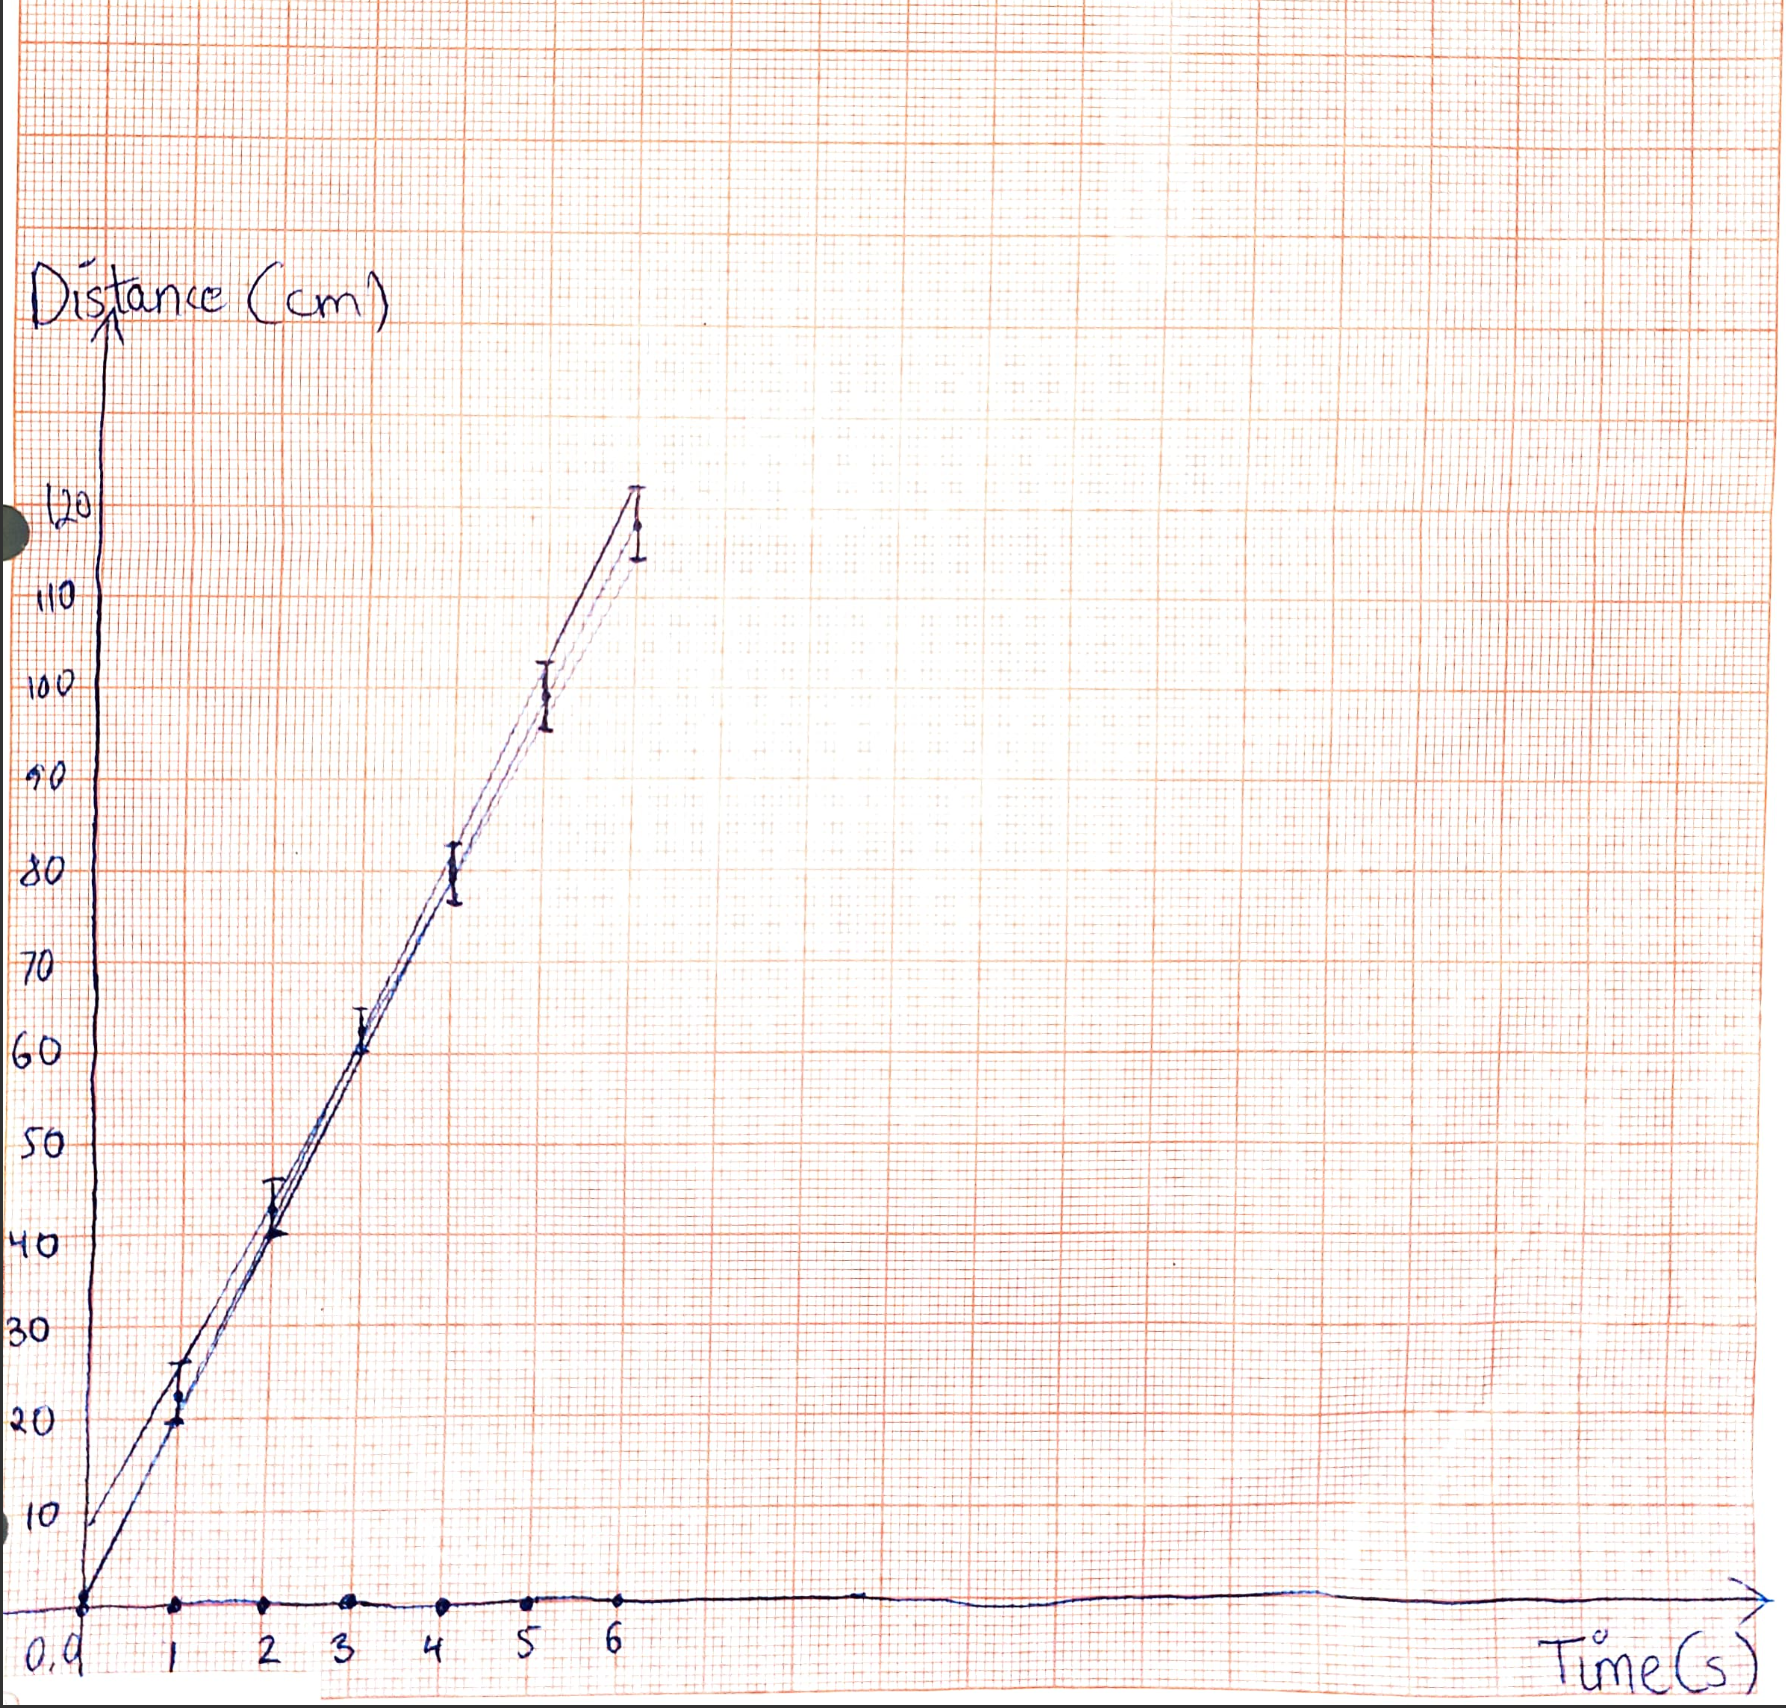
\includegraphics[width=0.75\linewidth]{graph.png}
\subsection{Line of Best Fit}
To calculate the slope of the line of best fit, we will take 2 points $(6,118)$ and $(5,99)$ on the line and find the equation:

\[
m = \frac{y_2 - y_1}{x_2 - x_1} = \frac{99 - 118}{5 - 6} = \frac{-19}{-1} = 19
\]

\[
y - y_1 = m(x - x_1)
\]

Substituting $(6, 118)$ and $m = 19$:

\[
y - 118 = 19(x - 6)
\]
Thus, we have our line of best fit
\[
y = 19x + 4
\]

\subsection{Line of Maximum Slope}
To calculate the slope of the line of maximum slope, we take points $(6, 123.5)$ and $(1, 20)$

\[
m = \frac{y_2 - y_1}{x_2 - x_1} = \frac{20 - 123.5}{1 - 6} = \frac{-103.5}{-5} = 20.7
\]

\[
y - y_1 = m(x - x_1)
\]

Substituting $(6, 123.5)$ and $m = 20.7$:

\[
y - 123.5 = 20.7(x - 6)
\]

Thus, our line of maximum slope is:

\[
y = 20.7x - 0.7
\]

\subsection{Line of Minimum Slope}
To calculate the slope of the line of maximum slope, we take points $(1, 26)$ and $(6, 115)$

\[
m = \frac{y_2 - y_1}{x_2 - x_1} = \frac{115 - 26}{6 - 1} = \frac{89}{5} = 17.8
\]

\[
y - y_1 = m(x - x_1)
\]

Substituting $(1, 26)$ and $m = 17.8$:

\[
y - 26 = 17.8(x - 1)
\]

\[
y = 17.8x + 8.2
\]

\section{Answer to Question 5.1}

The toy car manufacturer claims that the car moves at a speed of $20cm/s$. Our line of best fit has a slope of 19, indicating that the toy has a speed of $19 cm/s$. The maximum slope is 20.7 and the minimum slope is 17.8. Thus the uncertainty in the speed of the toy car is $\pm 1.45m/s$ Thus we can say that the speed of the car as calculated by our experiment is $19 \pm1.5 m/s$. This indicates that the claim is fairly correct.



\end{document}